\subsection{Optimisation settings and algorithms}
\label{subsec:poise__settings}

Once the user has defined a routine, it can then be run from the TopSpin command line using the command \texttt{poise ROUTINE\_NAME}.
However, the routine itself merely controls what parameters are being optimised: it does not specify what experiment is to be run (i.e.\ the pulse programme), nor any of the other parameters in the experiment.
These must be set by the user, and can most conveniently be stored in a TopSpin parameter set which can simply be loaded before starting the optimisation.
This flexibility means that the same \textit{type} of optimisation may be applied to different pulse sequences without having to create individual routines for each: for example, an experiment to optimise the NOE mixing time (as described in \cref{subsec:poise__noe}) can be run with different versions of the NOESY sequence depending on what is most appropriate.
Likewise, parameters such as the number of scans can be adjusted in order to run optimisations on samples with different concentrations.

Once the experiment parameters have been set up, there are a few more options which control how the optimisation is carried out:

\begin{itemize}
    \item the \texttt{--maxfev} option allows the user to control the maximum number of function evaluations, or in other words, the maximum number of experiments run.
        If the optimisation has not converged after acquiring this many spectra, the best result so far is simply returned.
        This effectively allows the time spent on optimisation to be capped.

    \item the \texttt{--quiet} option silences all output from the optimiser (the best parameters found are stored in the dataset itself after the optimisation ends, and can therefore be retrieved).
        This is useful when a POISE optimisation is to be run under automation.
        
    \item the \texttt{--separate} option allows each function evaluation to be run in a new experiment number, so that the optimisation trajectory can be analysed after its conclusion.

    \item perhaps most importantly, the \texttt{--algorithm} option allows the user to choose one of three optimisation algorithms: the \acf{nm} method\autocite{Nelder1965TCJ}, the \acf{mds} method\autocite{Torczon1989,DennisJr1991SIAMJO}, and the Py-BOBYQA trust region method\autocite{Powell2009Proc,Cartis2019ACMTMS}.
        All of these are derivative-free algorithms in that they do not use the value of $\nabla f$ at any point: as described in \cref{subsec:pureshift__optim_techniques}, gradients cannot be accurately estimated when there is noise in the cost function.%
        \footnote{Nocedal and Wright\autocite{Nocedal2006} give an upper bound on the finite difference gradient (as compared to the true gradient) of $\eta(x;\varepsilon)/\varepsilon + O(\varepsilon^2)$, where $x$ is the point at which the gradient is being measured, $\varepsilon$ is the step size used for the finite difference calculation, and $\eta(x;\varepsilon)$ is the noise in the region $[x - \varepsilon, x + \varepsilon]$. If $\varepsilon$ is small, the first term (the error due to noise) is large, and if $\varepsilon$ is large, the second term (the error due to the finite difference approximation) is large.}
        I will now describe these algorithms in slightly greater detail.
\end{itemize}

The NM method is a highly popular derivative-free optimisation algorithm, which maintains a set of points $\{y_1, y_2, \cdots, y_{n+1}\}$ during the optimisation, where $n$ is the number of parameters being optimised.
The convex hull of these points, $Y$, is the smallest possible set of points containing all the $y_k$ such that
\begin{equation}
    \label{eq:convex_hull}
    \forall x_1, x_2 \in Y, \forall \alpha \in [0, 1], \alpha x_1 + (1 - \alpha) x_2 \in Y,
\end{equation}
and is called a \textit{simplex}.
To provide an analogy for $n = 2$, the convex hull is the shape obtained by stretching a rubber band around three pins placed at $y_1, y_2, y_3$.
If this convex hull is nonempty---or equivalently, if the $n$ vectors $y_k - y_1$ ($2 \leq k \leq n + 1$) are linearly independent---then the simplex is called \textit{nonsingular}.
(In the $n = 2$ case, the convex hull would be empty if the three points were collinear.)

\begin{figure}[htb]
    \centering
    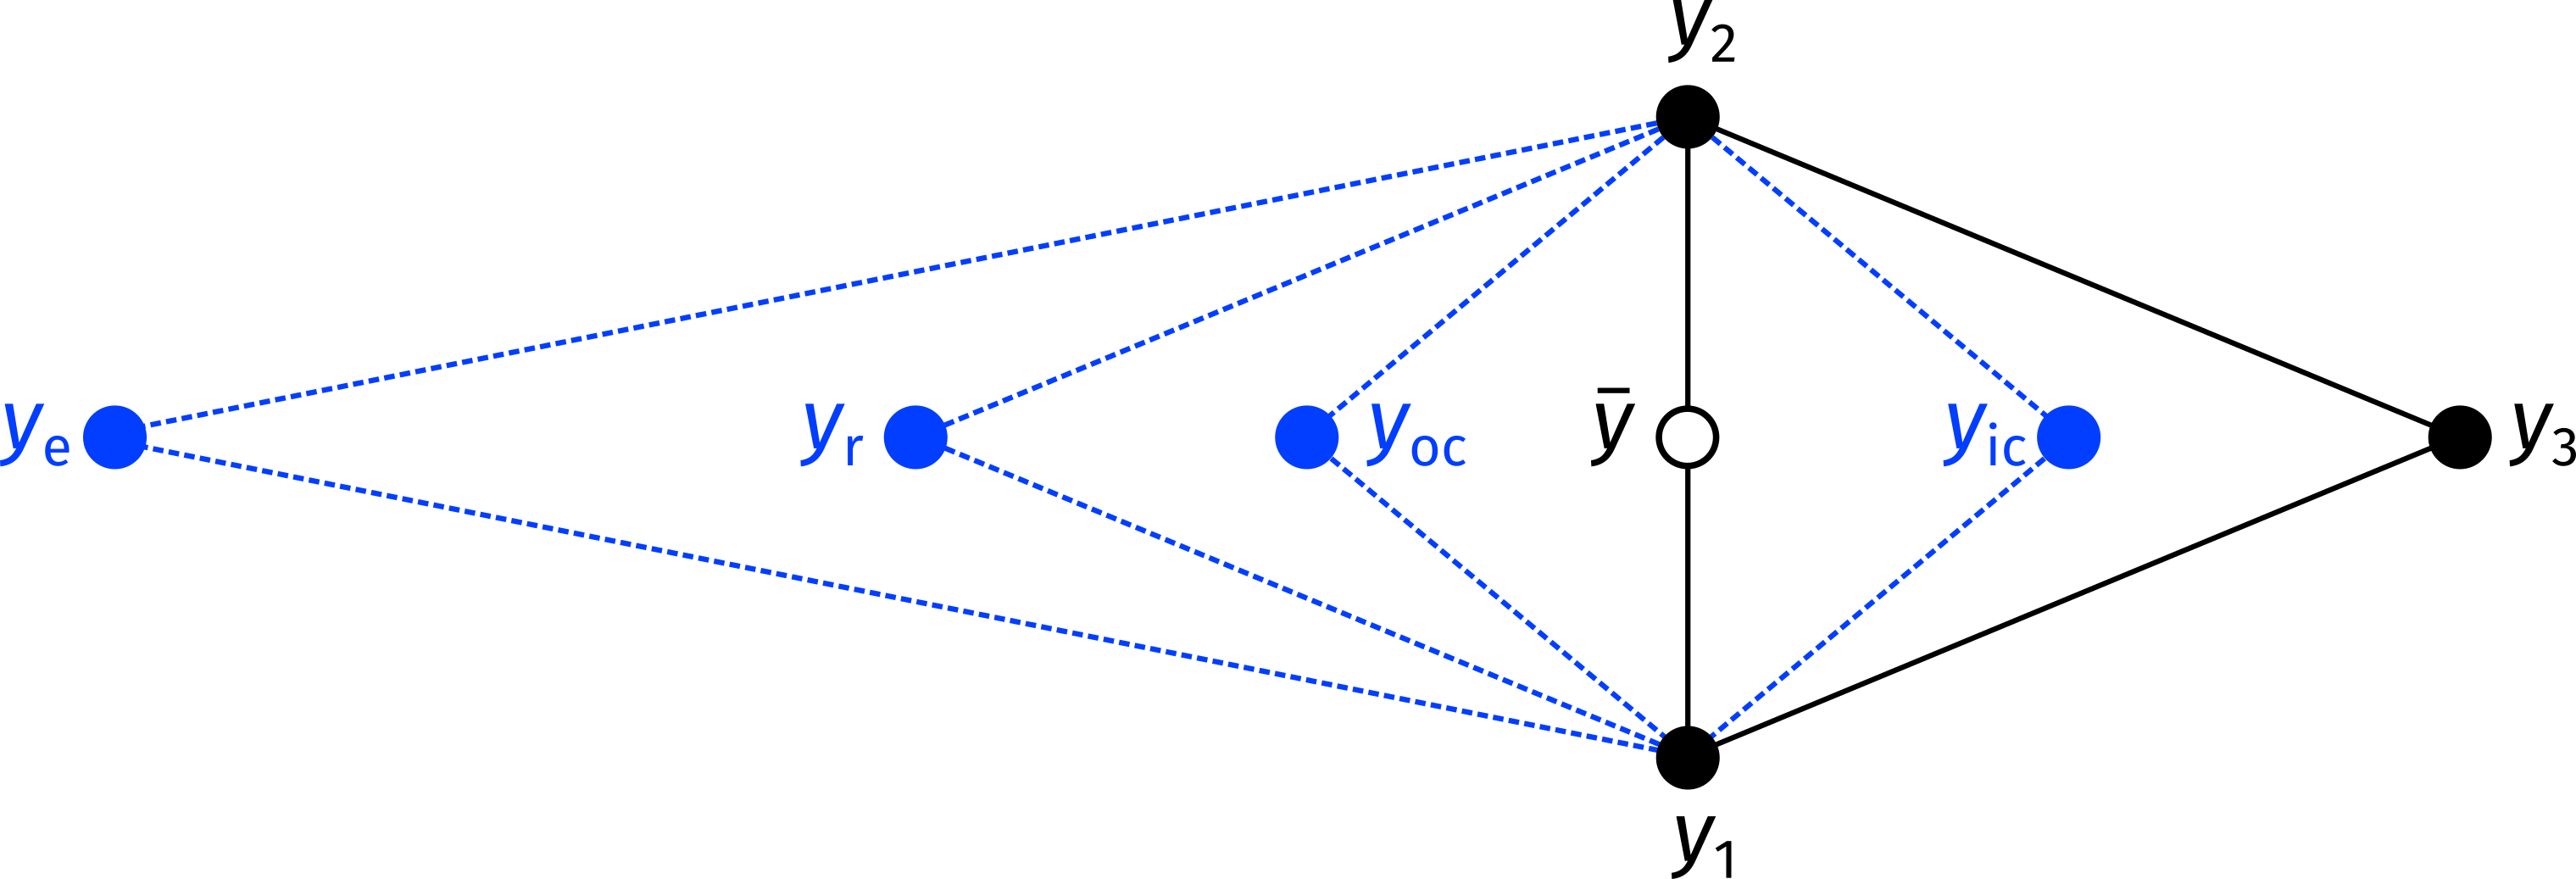
\includegraphics[draft=false]{poise/neldermead.png}
    \caption[Trial points in an iteration of the Nelder--Mead algorithm]{
        Diagram showing various points evaluated in one iteration of the Nelder--Mead algorithm (for an optimisation of two parameters).
        The solid black lines indicate the current simplex, which is assumed to be ordered such that $y_1$ is the best point (has the lowest cost function value) and $y_3$ the worst.
        The blue dots indicate the trial points which the algorithm attempts to replace $y_3$ with, and are further discussed in the text.
        Blue dashed lines indicate the simplex which would result if the corresponding trial point is accepted.
    }
    \label{fig:neldermead}
\end{figure}

The NM algorithm is in fact quite intuitive to understand.
The optimisation begins by measuring the cost function $f$ at every point of the simplex, and sorting the points in ascending order of cost function values (i.e.\ from best to worst), such that $f(y_1) \leq f(y_2) \leq \cdots \leq f(y_{n+1})$.
The centroid of the simplex is defined by the best $n$ points,
\begin{equation}
    \label{eq:simplex_centroid}
    \bar{y} = \sum_{i=1}^n y_i.
\end{equation}
On each iteration of the NM algorithm, we attempt to replace the worst point $y_{n+1}$  with a better point (\cref{fig:neldermead}).
The search for the new point is performed in several steps: first, the worst point is \textit{reflected} about the centroid of the simplex to obtain a new point:
\begin{equation}
    \label{eq:nm_reflect}
    y_\text{r} = \bar{y} - (y_{n+1} - \bar{y}).
\end{equation}
The value of the cost function is evaluated at this point, and is critical in determining how the algorithm proceeds.
If this reflected point falls in the middle of the pack, such that $f(y_1) \leq f(y_\text{r}) < f(y_n)$, this represents a `modest' improvement in the cost function: we simply replace the worst point with this and continue to the next iteration.

On the other hand, if the reflected point is better than all the other points (i.e.\ $f(y_\text{r}) < f(y_1)$), then we ambitiously attempt to \textit{expand} the simplex even further in that direction:
\begin{equation}
    \label{eq:nm_expand}
    y_\text{e} = \bar{y} - 2(y_{n+1} - \bar{y}).
\end{equation}
Of course, there is no guarantee that this is necessarily better than $y_\text{r}$; therefore, we choose whichever point of $y_\text{r}$ or $y_\text{e}$ had a lower value of $f$, and replace the worst point with this and continue to the next iteration.

If the reflected point is an improvement on the worst point but is no better than the remaining points, in that $f(y_n) \leq f(y_\text{r}) < f(y_{n+1})$, then the algorithm performs an \textit{outside contraction}, which resembles a half-hearted reflection:
\begin{equation}
    \label{eq:nm_outside_contract}
    y_\text{oc} = \bar{y} - (1/2)(y_{n+1} - \bar{y}).
\end{equation}
Conversely, if the reflected point is even worse than the worst point ($f(y_{n+1}) \leq f(y_\text{r})$), then this suggests that that search direction is very poor: we thus perform an \textit{inside contraction}, which uses a point halfway between the worst point and the centroid:
\begin{equation}
    \label{eq:nm_inside_contract}
    y_\text{oc} = \bar{y} + (1/2)(y_{n+1} - \bar{y}).
\end{equation}
If either of these contracted points are any better than $y_\text{r}$, then we replace the worst point in the simplex and continue to the next iteration; otherwise, we conclude that no search direction was good, and simply shrink the simplex towards the current best point by replacing each point $y_k$ with $(y_k + y_1)/2$.
In practice, these `last-resort' shrink steps occur very rarely.

\todo{Convergence... self implementation instead of using scipy}

In the preceding discussion, we noted that the simplex $Y$ was nonsingular if the $n$ vectors $y_k - y_1$ were linearly independent.
Equivalently, the matrix $M$ formed by concatenating these vectors
\begin{equation}
    \label{eq:simplex_matrix}
    M = \begin{pmatrix}
        y_2 - y_1, y_3 - y_1, \cdots, y_{n+1} - y_1 \\
    \end{pmatrix}
\end{equation}
must be nonsingular, i.e.\ have a nonzero determinant.
We can quantify how `close' the simplex $Y$ is to being singular, using the $l^2$ condition number of the matrix $M$, which in this context is usually referred to as the \textit{simplex condition}:
\begin{equation}
    \label{eq:simplex_condition}
    \kappa(Y) = \lVert M \rVert \lVert M^{-1} \rVert,
\end{equation}
where $\lVert M \rVert$ is the matrix norm induced by the Euclidean norm,
\begin{equation}
    \label{eq:matrix_norm}
    \lVert M \rVert = \max_{x \neq 0} \frac{\lVert Mx \rVert}{\lVert x \rVert}.
\end{equation}
A singular simplex $Y$ of course does not have a well-defined condition, since $M^{-1}$ does not exist.
However, the larger the condition of a simplex is, the closer it is to being singular.
Very loosely speaking, a long and thin simplex has a large condition number, and would be singular if its width were to go to zero.

The simplex updates made in the process of the NM algorithm mean that the simplex condition changes throughout the course of the optimisation.
If the simplex condition gets too large, it is possible that the optimisation will stall at a nonstationary point, since the search directions of the simplex are severely limited.
The MDS algorithm was proposed partially for the purpose of avoiding this ill-conditioning.\footnote{The main reason was in fact to better exploit computer parallelism, but it was also noticed that the MDS method proved to be generally more robust than NM.}
The MDS method is also simplex-based, but instead of reflecting a single worst point $y_{n+1}$ about the other points, it reflects all of the $n$ worst points $\{y_2, y_3, \cdots, y_{n+1}\}$ about the best point $y_1$.
This means that the shape of the simplex, and thus its condition number, is always preserved; from this, it could be concluded that at least one of the search directions was bounded away from being orthogonal to the gradient.\autocite{Torczon1989}
In simpler terms, at least one of the search directions is `good enough'.
